\documentclass[newpage]{homework}
\newcommand{\hwname}{Zooey Nguyen}
\newcommand{\hwemail}{zooeyn@ucla.edu}
\newcommand{\hwclass}{CS 146}
\newcommand{\hwtype}{Homework}
\newcommand{\hwnum}{1}
\usepackage{siunitx}
\begin{document}
\maketitle


\question
\begin{alphaparts}
    \questionpart \[\begin{bmatrix}2&2&3\end{bmatrix} \begin{bmatrix}-1\\0\\2\end{bmatrix}	= -2 + 0 + 6 = \boxed{4}\]
    \questionpart $\lVert x \rVert_1	=	2 + 2 + 3 = \boxed{7}$, $\lVert y \rVert_1	=	-1 + 0 + 2 = \boxed{1}$
    \questionpart $\lVert x \rVert_2	=	\sqrt{4+4+9} = \boxed{\sqrt{17}}$, $\lVert y \rVert_2	=	\sqrt{1+0+4} = \boxed{\sqrt{5}}$
    \questionpart Use dot product.
    \begin{align*}
        x \vdot y &= \lVert x \rVert_2 \lVert y \rVert_2 \cos{\theta} \\
        4 &=    \sqrt{17 \vdot 5} \cos{\theta}  \\ 
        \cos{\theta}    &=  \boxed{\frac{4}{\sqrt{85}}}    \\
    \end{align*}
\end{alphaparts}


\question
Note overall probability of defectiveness is $P(defective) = (0.25)(0.05) + (0.35)(0.04) + (0.40)(0.02) = 0.0345$
\begin{align*}
    P(A|defective)	&=	P(defective|A)P(A) / P(defective)	\\
                    &=	(0.05)(0.25) / (0.0345)	\\
                    &=  \boxed{0.362}  \\
    P(B|defective)	&=  (0.35)(0.04)  / (0.0345)	\\
                    &=  \boxed{0.405}  \\
    P(C|defective)	&=	(0.40)(0.02) / (0.0345)	\\
                    &=  \boxed{0.232}  \\
\end{align*}


\question
\begin{alphaparts}
    \questionpart \begin{align*}
        E[X+Y]	&=	\Sigma_x \Sigma_y x + y P(x,y)	\\
                &=  \Sigma_x \Sigma_y x P(x,y) + \Sigma_x \Sigma_y y P(x,y)   \\
                &=  \boxed{E[X] + E[Y]}
    \end{align*}
    \questionpart \begin{align*}
        Var[X+Y]	&=	\Sigma_x \Sigma_y [(x + y) - E[X+Y]]^2 P(x,y)	\\
        &=  \Sigma_x \Sigma_y [x + y - E[X] - E[Y]]^2 P(x,y)   \\
        &=  \Sigma_x \Sigma_y [(x - E[X]) + (y - E[Y])]^2 P(x,y)   \\
        &=  \Sigma_x \Sigma_y (x - E[X])^2 P(x,y) + \Sigma_x \Sigma_y (y - E[Y])^2 P(x,y)  + 2 \Sigma_x \Sigma_y (x - E[X])(y - E[Y]) P(x,y) \\
        &=  Var[X] + Var[Y] + 2 Cov[X,Y]    \\
        &=  \boxed{Var[X] + Var[Y]}
    \end{align*}
\end{alphaparts}


\question
\begin{alphaparts}
    \questionpart
        \begin{align*}
            E[Ax+b] &=	E[Ax] + E[b]	\\
                    &=  \boxed{AE[x] + b}
        \end{align*}
    \questionpart 
        \begin{align*}
            Cov[Ax+b]	&=	E[(Ax + b - E(Ax + b))(Ax + b - E(Ax + b))^T] \\
            &=  E[(Ax + b - AE[x] - b)(Ax + b - AE[x] - b)^T] \\
            &=  E[A(x - E[x])A^T(x - E[x])^T] \\
            &=  AA^T E[(x - E[x])(x - E[x])^T] \\
            &=  \boxed{AA^T Cov[x]}
        \end{align*}
    \questionpart $y$ will be a multivariate Gaussian with expectation $AE[x] + b$ and covariance matrix $AA^T Cov[x]$ as seen from previous parts.
\end{alphaparts}

\question
\begin{alphaparts}
    \questionpart Done in Python. Red and green indicate the two possible outcomes for each applicant. The 2031 admissions data is linearly separable while the 2030 data is not.
    \begin{figure}[h]
        \centering
        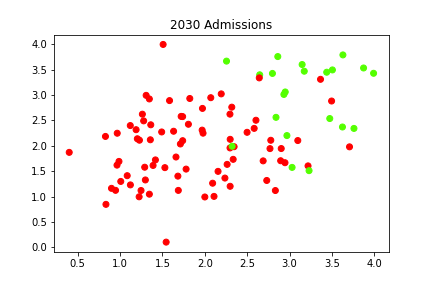
\includegraphics[width=0.6\textwidth]{5ai.png}
    \end{figure}
    \begin{figure}[h]
        \centering
        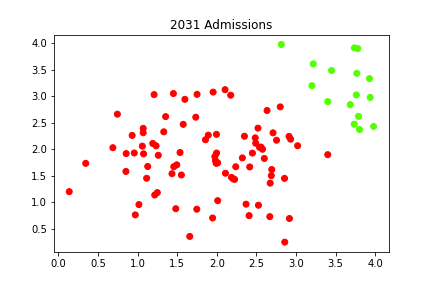
\includegraphics[width=0.6\textwidth]{5aii.png}
    \end{figure}

    \questionpart For 2030 admissions. The algorithm did not converge and clearly had a wrong answer at the end since the data is not linearly separable.
        \begin{itemize}
            \item   Weights: [6.17445 -1.46852]
            \item   Bias: -31
        \end{itemize}
        For 2031 admissions. The algorithm did converge and from the plot we can see it did separate the data, however it did not optimise for the margin as expected from what we've seen before.
        \begin{itemize}
            \item Weights: [4.53609 2.42091]
            \item Bias: -22
        \end{itemize}
        \begin{figure}[h]
            \centering
            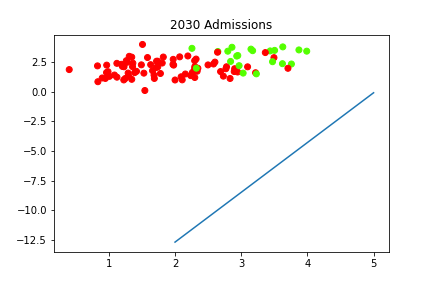
\includegraphics[width=0.6\textwidth]{5bi.png}
        \end{figure}
        \begin{figure}[h]
            \centering
            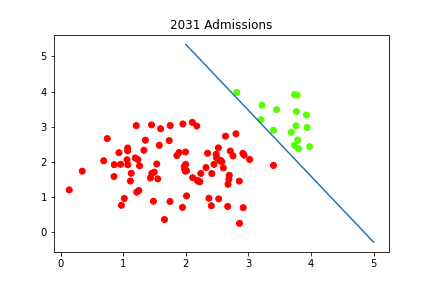
\includegraphics[width=0.6\textwidth]{5bii.png}
        \end{figure}
    \questionpart The point closest to the hyperplane in the 2031 dataset is at (3.2, 3.2) at a distance of 0.051 from the plane.
\end{alphaparts}


\end{document}
